\documentclass[12pt,letterpaper]{article}

\usepackage[utf8]{inputenc}
\usepackage[T1]{fontenc}
\usepackage{amsmath}
\usepackage{amsfonts}
\usepackage{amssymb}
\usepackage{amsthm}
\usepackage[left=2cm,right=2cm,top=2cm,bottom=2cm,headheight=22pt]{geometry}
\usepackage{fancyhdr}
\usepackage{setspace}
\usepackage{lastpage}
\usepackage{graphicx}
\usepackage{caption}
\usepackage{subcaption}
\usepackage{paralist}
\usepackage{url}

\theoremstyle{definition}
\newtheorem{question}{Question}
\newtheorem{example}{Example}
\newtheorem{exercise}[question]{Exercise}
\newtheorem*{challenge}{Challenge}
\newtheorem*{theorem}{Theorem}
\newtheorem*{definition}{Definition}

\begin{document}

%Paramètres de mise en forme des paragraphes selon les normes françaises
\setlength{\parskip}{1ex plus 0.5ex minus 0.2ex}
\setlength{\parindent}{0pt}

%Paramètres relatifs aux en-têtes et pieds de page.
\pagestyle{fancy}
\lhead{Theron J Hitchman}
\chead{\Large Reading and Guided Practice \#02}
\rhead{Spring 2016}
\lfoot{\emph{Math and Decision Making }}
\cfoot{}
\rfoot{\emph{\thepage\ of \pageref{LastPage}}}

\section*{Introduction}

In this reading, we will see some new vocabulary to help us talk about graphs and their structure, and learn a theorem.

\section*{Goals}
At the end of this assignment, a student should be able to:
\begin{compactitem}
\item Discuss what makes a graph.
\item Use the terms \emph{isomorphism}, \emph{planar}, \emph{loop}, and \emph{drawing} properly.
\item State and use \emph{Euler's Formula} appropriately.
\end{compactitem}
A student might also be able to:
\begin{compactitem}
\item Describe why there is no planar drawing of $K_5$, the complete graph on five vertices.
\item Decide if the bipartite graph $K_{3,3}$ is planar or not.
\end{compactitem}

\section*{Reading and Questions for Graph Theory Meeting Three}

You may have noticed that mathematics uses a lot of specialized vocabulary.
For someone new to a particular bit of math, this can be a challenge: there are so many new words
it can be hard to keep them straight.
So, this might seem like what makes mathematics hard. (It is sometimes.)
But it is also what makes mathematics \emph{possible}. 
Each vocabulary word is an \emph{abstraction} --- a whole bundle of ideas wound up into a single unit.

This reading has lots of vocabulary words in it. It is my belief that if you can see each word as connected
to the ideas it represents, things will be easier. 
Right now, our most important vocabulary word is \emph{graph}.

\subsection*{Some Technicalities About Graphs}

We have decided that the word \emph{graph} stands for a thing consisting of two related collections:
first, we must have a collection of things, which we will call \emph{vertices}; second, we must have a
collection of relations between pairs of things, which we will call \emph{edges}.

Here is one tricky bit. How can we use the idea of an edge? More specifically, can an edge be a relationship
between a single vertex and itself, or must it connect two distinct vertices? Well this depends on the
situation. Some people allow for edges which join a vertex to itself, and some do not. By the way, an edge
which starts at a vertex and then comes back to that vertex is called a \emph{loop}. 
(Try drawing a simple example. You will see that this is a good choice of term.) So, the question can be restated:
Will the term \emph{graph} allow loops or not?

There really is a choice to be made here. Sometimes allowing loops is helpful, sometimes it makes things more 
complicated. For our purposes, we just have to make a choice and live with it. So, I declare this: we will
not allow loops. \textbf{A graph may not have an edge which starts and ends at the same vertex. 
That is, it may not contain loops.}

\begin{exercise}
Check that the complete graph on five vertices does not have any loops. (Hint: review the last reading
if you do not recall what the complete graph on five vertices is.)
\end{exercise}


\subsection*{Connectedness and Components}

Below is a drawing of a graph.

\begin{figure}[h]
\centering
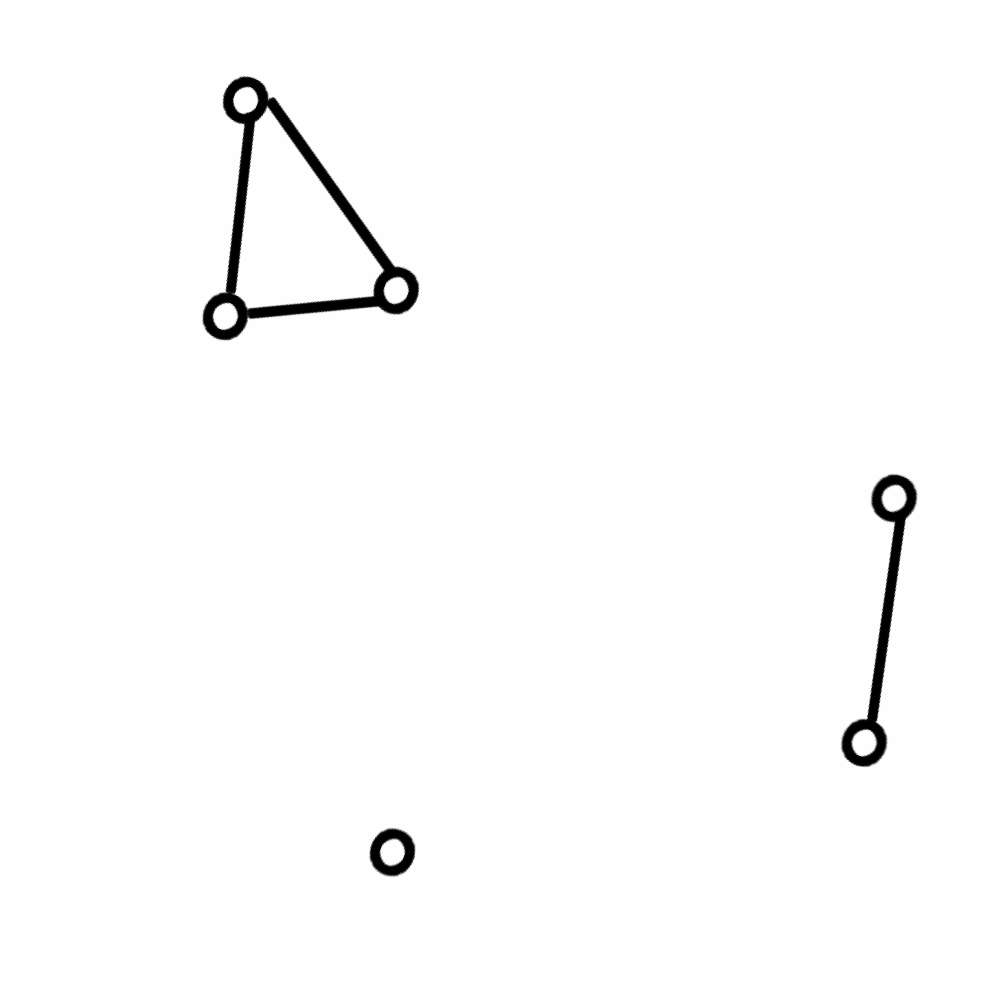
\includegraphics[width=.5\textwidth]{images/disconnected.png}
\caption{This is a single graph!}
\label{figure:disconnected}
\end{figure}

Do you find that odd in any way? Note that I said ``a graph,'' not three graphs. But there are clearly 
three distinct pieces.

What is happening is that this graph fails to be \emph{connected}. We say a graph is connected when
for each pair of vertices, there is a chain of edges that you can use to go between that pair of vertices.

That fails in Figure \ref{figure:disconnected} because we can choose some pairs of vertices with no such 
chain of edges. For example, the lone vertex near the bottom of the drawing has NO edges coming out of
it at all, so it cannot be connected to any other vertex by a chain of edges.

This particular graph has three pieces, each of which is a sort of ``maximally connected sub-graph.''
Each such piece is called a \emph{connected component} of the graph (or just a \emph{component} for short).
Our graph has three components: one that looks like a triangle, one that looks like a line segment, and one that 
is a lonely vertex.

This is a spot which is easy to trip over. A graph can have lots of pieces (components), which makes it look
like a collection of several graphs sitting next to each other. Be careful about this.

\begin{exercise}
Draw an example of a connected graph.
\end{exercise}

\begin{exercise}
Draw an example of a disconnected graph which is different from the one I drew in 
Figure \ref{figure:disconnected}.
\end{exercise}

\subsection*{Drawings and Isomorphisms}

By now we have seen several examples of graphs. Here are two that you probably have seen before.
(Careful, I am going to draw them next to each other to save space on the page, but this is really TWO graphs,
not one graph with two components.)

\begin{figure}[h]
\centering
\begin{subfigure}[b]{0.4\textwidth}
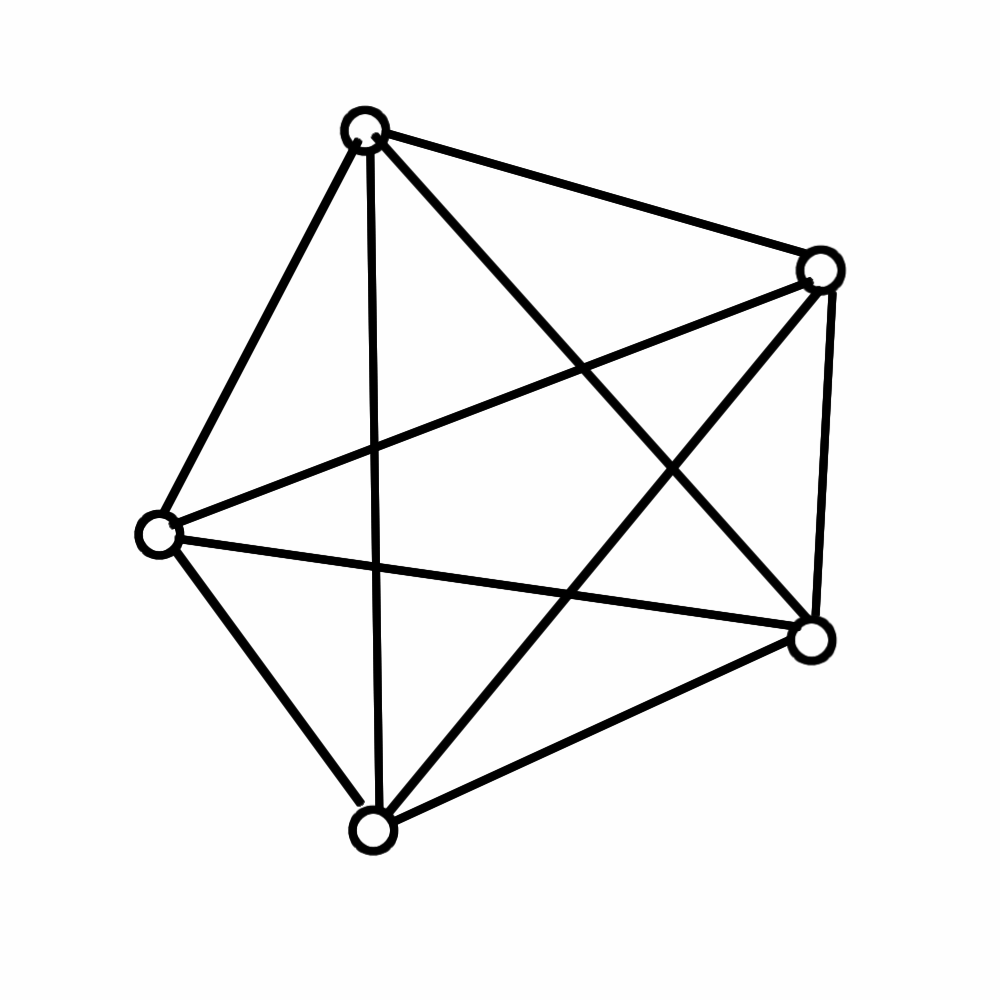
\includegraphics[width=\textwidth]{images/k5.png}
\caption{The standard drawing of $K_5$}
\label{figure:stdK5}
\end{subfigure}
\begin{subfigure}[b]{0.4\textwidth}
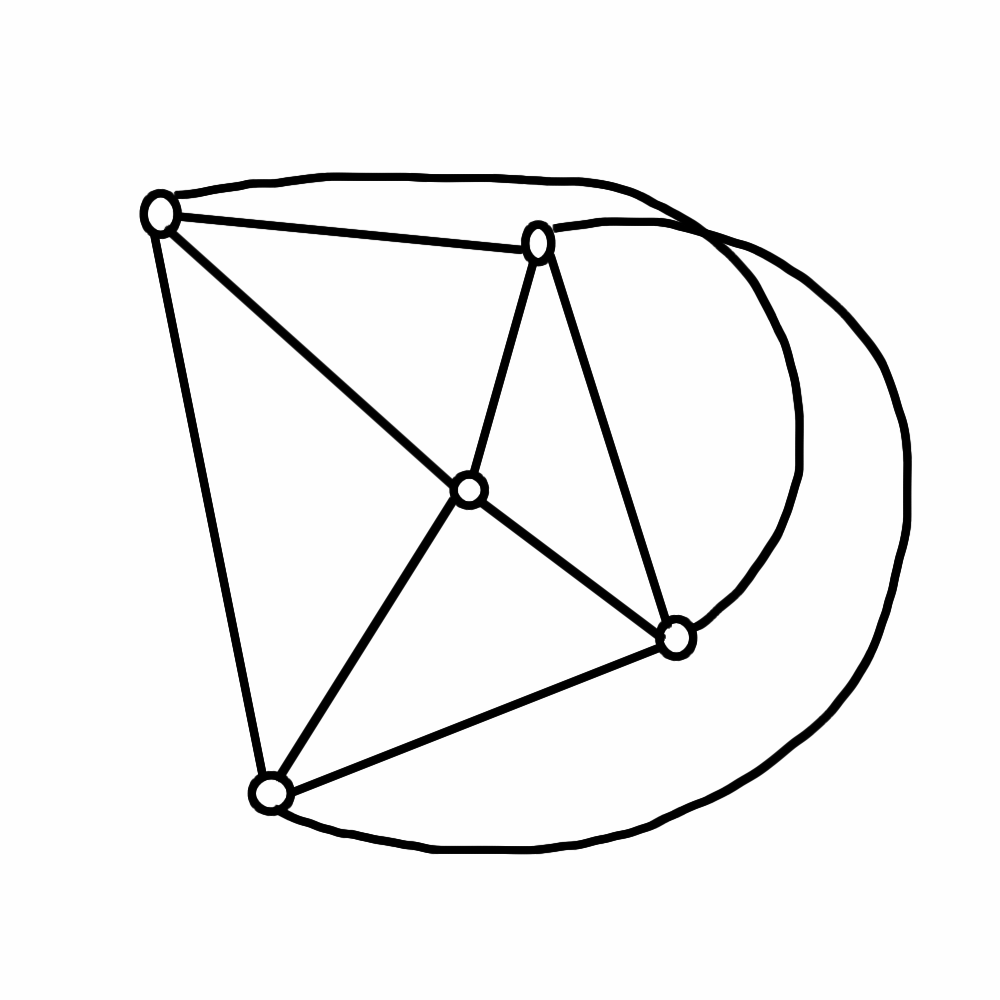
\includegraphics[width=\textwidth]{images/altk5.png}
\caption{A non-standard drawing of $K_5$}
\label{figure:altK5}
\end{subfigure}
\caption{Two drawings of $K_5$}
\label{figure:K5s}
\end{figure}

\begin{exercise}
Convince yourself that these are really ``the same graph.''
\end{exercise}

What do we really mean by ``the same graph?'' Well, the idea is that the relationships represented by the graph
Figure \ref{figure:stdK5} are the same as the relationships represented by the graph in Figure \ref{figure:altK5}.
In both cases, the graph tells us that there are five things, and each of the five things is related to each of
the other four. In fact, each of these graphs is a different \emph{drawing} of the complete graph on five
vertices. This complete graph is important enough that mathematicians have given it a name. We call it
$K_5$. (That is not quite as cool as BB-8.)

The kind of relationship where two graphs are really the same thing is called \emph{isomorphism}, and
we call the pair of graphs under consideration \emph{isomorphic}. This funny word derives from the
roots \emph{iso}, meaning same, and \emph{morph}, meaning shape or form.

To sum up, the graphs in Figure \ref{figure:stdK5} and Figure \ref{figure:altK5} are isomorphic, and both are
\emph{drawings} of our special friend $K_5$.

\begin{exercise}
Pick a graph which is different from $K_5$. Make two different looking drawings of that graph.
\end{exercise}

\begin{exercise}
Draw two graphs which are \textbf{definitely not} isomorphic. Write down an explanation for why they
are definitely different.
\end{exercise}

I hope it is clear to you that a single graph could have many different drawings, and those drawings will be 
isomorphic, but the way they are isomorphic might be really hard to see.

\subsection*{Planarity and Euler's Formula}

We began class by looking for a way to draw $K_5$, the complete graph on five vertices, in a way that involved
no crossing edges. This is pretty challenging. I hinted that not every graph has this property. This is 
important enough that it has a name.

A graph is called \emph{planar} when it is possible to make a drawing of the graph which has no edge
crossings.

If you recall, this is the same as saying that the graph has crossing number equal to zero.

\noindent
\textbf{Important Note to Dispel a Common Point of Confusion:} There is a distinction to be made here between 
a graph, and the different drawings of that graph. A single graph has many different drawings, of course. The word
planar gets applied to both, and we want to be careful.
\emph{A drawing is planar if it has no edge crossings.} You can 
see this just by looking.  \emph{A graph is planar if it has a drawing which is planar.} This is harder to check, 
because you have to either find a drawing which is planar, or somehow make an argument that there isn't any way
to do that.


\begin{exercise}
Remember some examples of planar graphs that you have seen so far. If you do not remember any, 
go back through examples from the previous readings and homework, and note which ones are 
definitely planar.
\end{exercise}

Back at the dawn of graph theory, one of its first practitioners (Leonard Euler, pronounced ``oil-er'')
found a really interesting fact about planar graphs. Nowadays, we write it down in a way to make it look
official:

\begin{theorem}[Euler's Formula for Planar Drawings of Planar Graphs] Suppose that we have a planar 
drawing of a planar graph. That is, a drawing of the graph where no edges cross. Let $V$ be the total number 
of vertices in the graph, and let $E$ be the total number of edges in the graph. The drawing of the graph 
divides the plane into a bunch of regions, including one region which lies completely outside the graph. 
Let $R$ be the total number of regions. Then
\[
V-E+R = 2
\]
\end{theorem}

We're not going to prove this right now. Instead, let's look at an example.

\begin{figure}[h!]
\centering
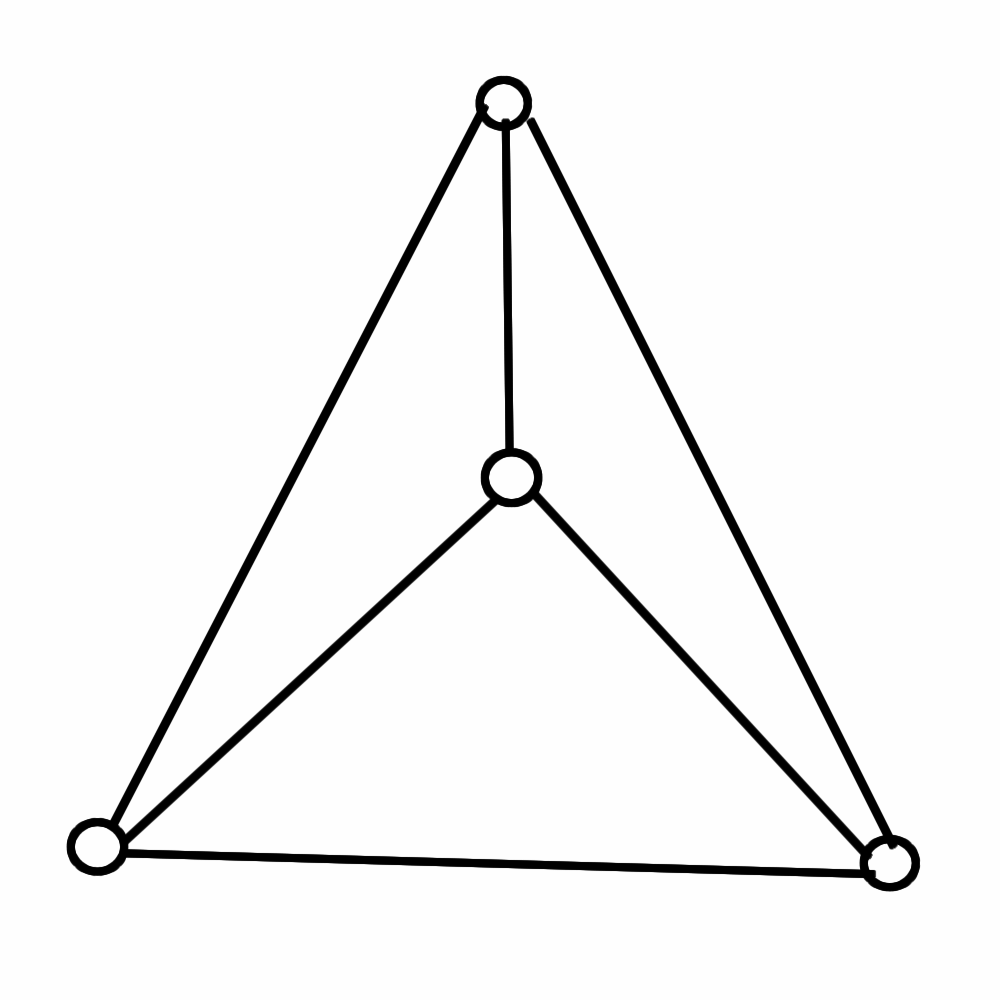
\includegraphics[width=.3\textwidth]{images/std_k4.png}
\caption{$K_4$, the complete graph on four vertices}
\label{figure:stdk4}
\end{figure}

For the graph in Figure \ref{figure:stdk4}, we have $V=4$, $E=6$ and $R=4$ (don't forget the one on the outside!). So, we can check Euler's formula works here.
\[
V - E + R = 4 - 6 + 4 = 2
\]

\begin{exercise}
Make drawings of three different planar graphs, so that there are no crossing edges. Check that
Euler's formula works for each.
\end{exercise}

\begin{challenge}
Can Euler's formula help you think about the Five Cities Puzzle? Or the Three Utilities Puzzle?
\end{challenge}

\subsection*{One Last New Name, and Some Hints}

The graph in the Three Utilities Puzzle is called the \emph{complete bipartite graph on three and three vertices},
and mathematicians call it by the name $K_{3,3}$. The idea here is that there are two groups of vertices, 
each with three vertices in it, and there are these edges: two vertices are connected by an edge exactly when they 
belong to different groups.

Here is a standard drawing of $K_{3,3}$.

\begin{figure}[h]
\centering
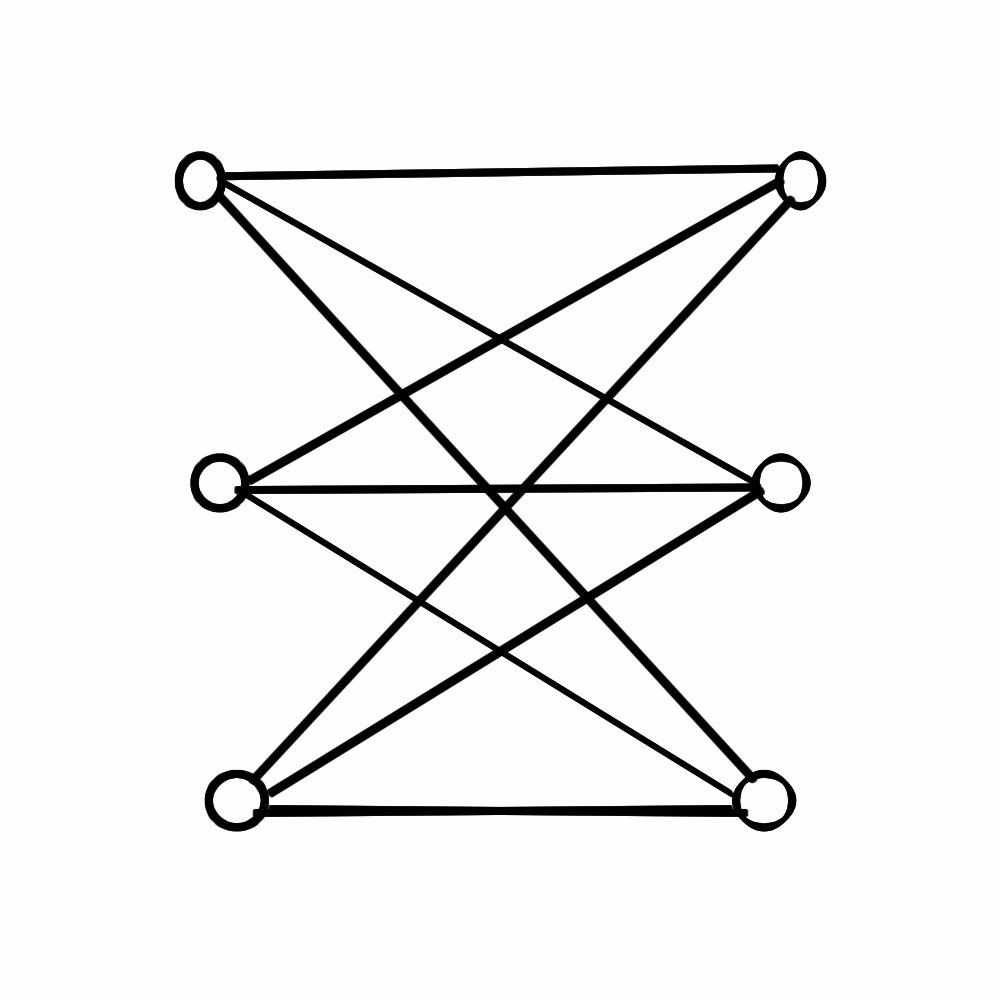
\includegraphics[width=.4\textwidth]{images/k3,3.png}
\caption{The complete bipartite graph graph $K_{3,3}$}
\label{figure:stdk33}
\end{figure}

The two puzzles we have considered so far can be restated in this way: Is $K_5$ planar? Is $K_{3,3}$ planar?

\begin{challenge}[Hint] Suppose a graph has a triangle in it. Consider all of the possibilities for putting down 
two more vertices either inside the triangle or outside the triangle. Can this help you solve the Five Cities
Puzzle?
\end{challenge}

\begin{challenge}[Hint] The graph $K_{3,3}$ does not have any triangles in it. But you can find a square!
What parts of what you did in the last challenge can be reused (adapted?) to the Three Utilities Puzzle?
\end{challenge}



%\begin{thebibliography}{9}
%\end{thebibliography}

\end{document}
%sagemathcloud={"zoom_width":100}


























